
\begin{figure}
	\centering
	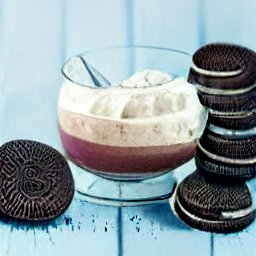
\includegraphics[width=.25\textwidth]{lasse/oreo_curd.jpg}\hspace{3mm}
	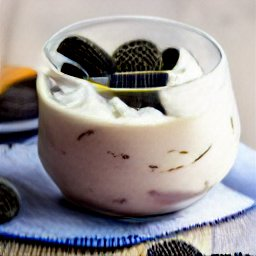
\includegraphics[width=.25\textwidth]{lasse/oreo_curd1.jpg}\hspace{3mm}
	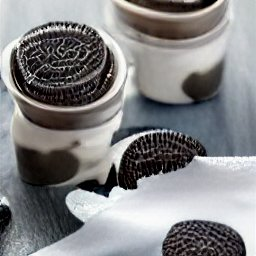
\includegraphics[width=.25\textwidth]{lasse/oreo_curd2.jpg}\hspace{3mm}
\end{figure}
    



\begin{recipe}
    [ % Optionale Eingaben
        preparationtime = {\unit[50]{min}},
        portion = \portion{6},
        %calory,
        source = Lasse (Malin)
    ]
    {Oreo Quark}
    
    \introduction{
        \# Kalorienbombe EXTREM
    }
    

    \ingredients
    {% Zutatenliste
        \unit[2]{Pkg} & Oreo Kekse \\
        \unit[250]{g} & Quark \\
        \unit[75]{g} & Puderzucker \\
        \unit[100]{g} & Frischkäse \\
        \unit[300]{ml} & Sahne \\
        \unit[2]{Pkg} & Paradiescreme Vanille 
    }
    
    \preparation
    { % Schrittweise Zubereitung
        \\
        Die Kekse 1 Tag vor der Zubereitung einfrieren. Die gefrorenen Kekse mit einer Keule je nach Geschmack fein oder grob zerdeppern.

        Quark, Puderzucker und Frischkäse gut verrühren. Die Sahne schlagen. Die Paradiescreme nach Packungsanleitung anrühren. Die Quarkmischung mit Paradiescreme verrühren und die Sahne unterheben.

        Nun abwechselnd die Creme mit den gemahlenen Keksen in eine Glasschüssel schichten, dabei mit einer Cremeschicht anfangen und mit einer Keksschicht aufhören.
    }
    
    \hint
        {% Hinweise
        Sollte man am besten kalt essen. Also eventuell nochmal eine Runde in den Kühlfrank. 
        
        Die Oreos müssen nicht unbedingt gefroren sein, das macht es nur leichter. 
        
        Die Bilder wurden von einer glücklichen KI generiert.
        }
    
    \end{recipe}
    